\subsection{Experimental Evaluation}

After profiling the performance of the perception and estimation algorithm and formulating the Robust MPC controller for the hex-rotor model (equation \ref{}), we experimentally evaluate the tracking performance and estimated energy consumption based on actual flights around a pre-defind trajectory. For comparision, we use a Model Predictive Controller (also coded in CVXGEN) with the same cost function and initial feasible sets as in our Robust MPC formulation. Comparision to such a controller would give a baseline to measure the benefits of our co-design method against the a similar control algorithm that does not leverage co-design and is unaware of the estimator algorithm that gives it a state estimate. Note, in our experimental evaluation, due to WHAT??? we did not use visual odometry for localization but simulate the behaviour of the visual odometry based estimation by adding a delay and norm bounded estimation error as profiled ($\forall i \mid (\delta_i,\epsilon_i) \in \Delta $) for the different Visual odometry modes to the VICON based measurements. 

For the evaluation, we fly in a predefined trajectory as shown in figure \ref{}, repeating the experiment 10 times to gather enough data to conclusively measure the performance of Robust MPC and MPC with fixed modes of ($\delta,\epsilon$). Note that since the controller was a sampled discrete-time controller working with simulated 20Hz camera updates, this realistically restricts us to using modes of estimator operation with delay ($\delta$) less than (1/20s), or one sampling period, i.e. modes corresponding to 50, 100, 150 and 200 maximum corners from the FAST detector (see figure \ref{}). These modes and their estimated power consumption is in table \ref{}.

\begin{table}[h]
\begin{tabular} {|c|c|c|c|c|}
	\hline
	Mode & \#C & $\epsilon$ & $\delta$ (ms) & $E[P]$(w) \\ \hline
	0 & 50 &  24.88 & 0.028 &  0.778  \\ \hline
 	1 & 100 & 29.82 & 0.0237 &  0.862  \\ \hline
	2 & 150 & 34.66 & 0.0230 & 0.870 \\ \hline
	3 & 200 & 38.01 & 0.0113 & 0.951 \\ \hline
	\end{tabular}
	\caption{Estimation modes used in the experiment. \#C represents maximum number of FAST corners requested, $\epsilon$ shows the worst case error bound on the state estimate, $\delta$ is the $90^{th}$ percentile execution time for that mode, and $E[P]$ represents the estimated power consumption in that mode as profiled offline.}
\end{table}



\begin{figure}[t]
	\centering
	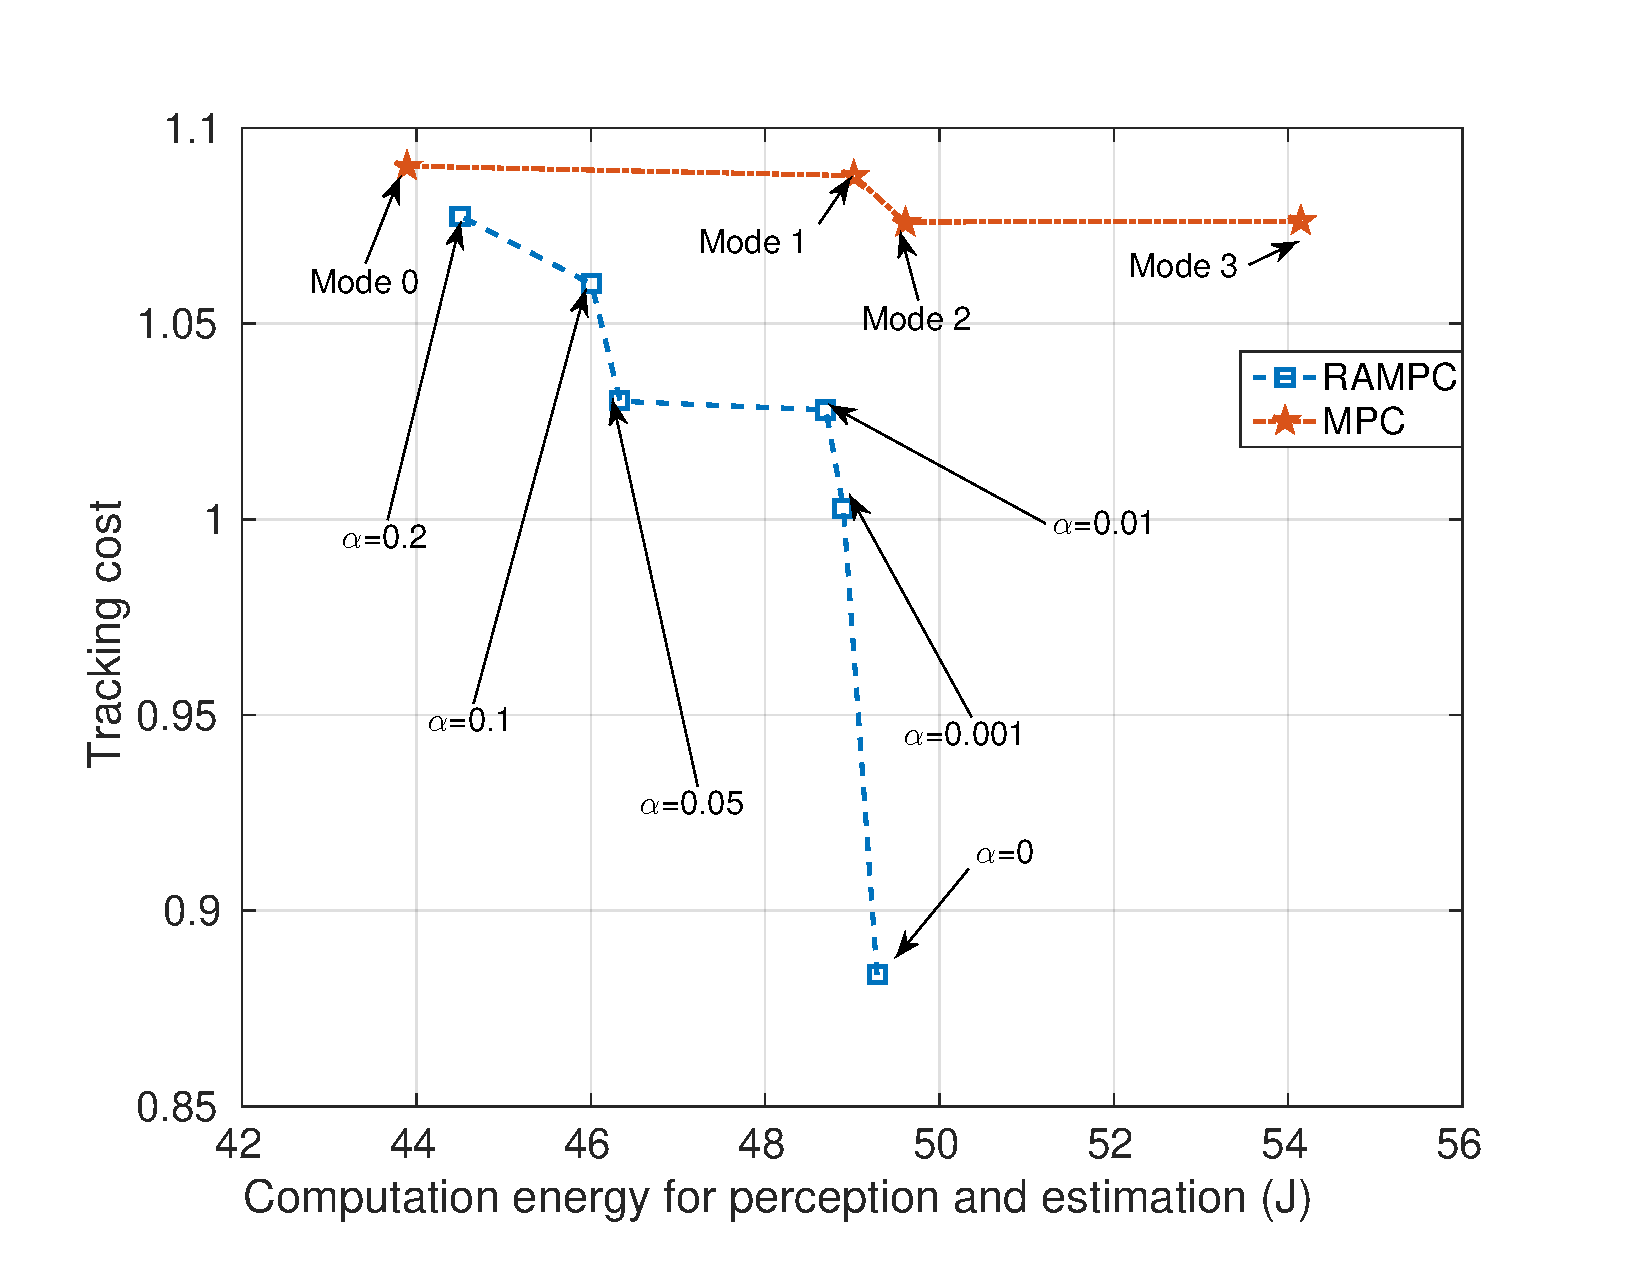
\includegraphics[width=0.49\textwidth,scale=0.7]{figures/TrackingVsEnergy}
        \vspace{-20pt}
	\caption{\small{Tracking cost vs estimated computation energy for executing the perception and estimation algorithm. Note for MPC, different energies are realized only by operating at different fixed modes of the perception and estimation algorithm. Using RAMPC as the controller, the different energies are due to run-time scheduling of different modes based on the optimal value of the cost function \ref{eq: } at each time step based on different values of $\alpha$. It is worth noting that RAMPC with co-design outperforms standard MPC on a tracking performance per unit energy throughout.}}
	\label{fig:modeSwitching}
\end{figure}


